%12.数学分析利用级数收敛来构造连续函数, 距离空间的完备化
\documentclass[main.tex]{subfiles}                                              
\begin{document}

\section{引言}

本章的中心主题是本书中所实践的 NURBS 几何与其他表示曲线和表面的方法之间的关系，以及在两个系统之间交换几何数据的几个重要标准格式。我们在整本书中使用了一种特定形式的节点向量；第 12.2 节讨论了另一种类型的节点向量及两种类型之间的转换。第 12.3 节描述了 NURBS 曲线和表面在三个标准(IGES、STEP 和 PHIGS)中的定义。我们指出，我们的 NURBS 与这些标准的 NURBS 兼容(唯一的例外是 IGES 和 PHIGS 允许不连续的曲线和表面)。最后，第 12.4 节提供了一些关于在 NURBS 系统与其他系统之间交换几何数据的一般指导。

\section{结点向量}
节点向量可以分为两组:固定和非固定；在每组中又有均匀和非均匀节点向量。以下是一些示例:

固定，均匀:

\[
\{ 0,0,0,0,1,2,3,4,4,4,4\}
\]

\[
\{  - {0.5}, - {0.5}, - {0.5},1,{2.5},4,4,4\}
\]

固定，非均匀:

\[
\{ 0,0,0,2,3,6,7,7,7\}
\]

\[
\{ 0,0,0,0,1,2,2,3,4,5,5,5,5\}
\]

非固定，均匀:

\[
{U}_{1} = \{  - 3, - 2, - 1,0,1,2,3,4,5\}
\]

\[
{U}_{2} = \{ 0,1,2,3,4,5,6,7,8,9,{10},{11}\}
\]

非固定，非均匀:

\[
\{ 0,0,1,2,3,4\}
\]

\[
\{  - 2, - 1,0,4,5,6,7\}
\]

因此，夹紧/未夹紧指的是第一个和最后一个节点值是否以等于度数加一的重数重复，而均匀/非均匀则指节点间距。要实现均匀且未夹紧，所有节点跨度必须长度相等。要实现均匀且夹紧，仅“内部”节点跨度必须长度相等。读者可能已经注意到，我们现在称之为夹紧、均匀和非均匀的内容，正是我们迄今为止称之为非周期性、均匀和非均匀的内容。在对未夹紧节点向量进行简要研究之后，我们将为这种术语在节点流中间的变化提供一个微弱的借口。由于本书中假设使用夹紧节点向量，因此在此无需进一步阐述。然而，在继续研究未夹紧节点向量之前，我们提供以下与夹紧节点向量相关的提醒:

\begin{itemize}
\item 如果我们给定一个具有 \(m + 1\) 个节点和端点重数为 \(p + 1\) 的夹紧节点向量，那么我们需要 \(n + 1\left( { = m - p}\right)\) 个控制点来定义一个 \(p\) 次曲线；也就是说，节点向量决定了曲线的度数、控制点的数量以及有效的参数范围；
\end{itemize}

\begin{itemize}
\item 从几何上讲，夹紧曲线可以是开放的或闭合的；如果一条曲线是闭合的，那么它是否以 \({C}^{k}\) 连续性闭合取决于第一个 \(k\) 和最后一个 \(k\) 个内部节点跨度，以及第一个 \(k + 1\) 和最后一个 \(k + 1\) 个权重和控制点。
\end{itemize}

现在考虑未夹紧的均匀节点向量 \({U}_{1}\) 。使用 Cox-deBoor 算法，方程 (2.5)，我们可以计算 \(8 - p\) 度 \(p\) 基函数，适用于 \(p =\)  \(0,\ldots ,7\) 。度为 2 和 3 的基函数，以及一条二次曲线和一条三次曲线，分别显示在图 12.1a 和 12.1b 中。节点位置标记在曲线上。注意，这些曲线在端点处并未夹紧，即它们的起始点和终点与控制点不重合。此外，在 \(u \in  \left\lbrack  {{u}_{i},{u}_{i + 1}}\right)\) 处评估曲线需要函数 \({N}_{i - p,p}\left( u\right) ,\ldots ,{N}_{i,p}\left( u\right)\) ；因此，这些曲线仅在参数范围 \(u \in  \left\lbrack  {{u}_{p},{u}_{m - p}}\right\rbrack\) 上定义，这与夹紧曲线的情况相同。因此，图 12.1a 的二次曲线在 \(u \in  \left\lbrack  {-1,3}\right\rbrack\) 上定义，而图 12.1b 的三次曲线在 \(u \in  \left\lbrack  {0,2}\right\rbrack\) 上定义。图 12.2 显示了如何使用未夹紧的均匀节点向量 \({U}_{2}\) 定义一条闭合的三次曲线。由于 \(m = {11}\) 和 \(p = 3\) ，我们需要八个控制点 \(\left( {n = 7}\right)\) 。我们在末尾环绕 \(p\left( { = 3}\right)\) 控制点；即 \({\mathbf{P}}_{5} = {\mathbf{P}}_{0},{\mathbf{P}}_{6} = {\mathbf{P}}_{1}\) 和 \({\mathbf{P}}_{7} = {\mathbf{P}}_{2}\) 。有效的参数范围是 \(u \in  \left\lbrack  {3,8}\right\rbrack\) 。这导致曲线闭合，并具有 \({C}^{2}\) 连续性。

\begin{center}
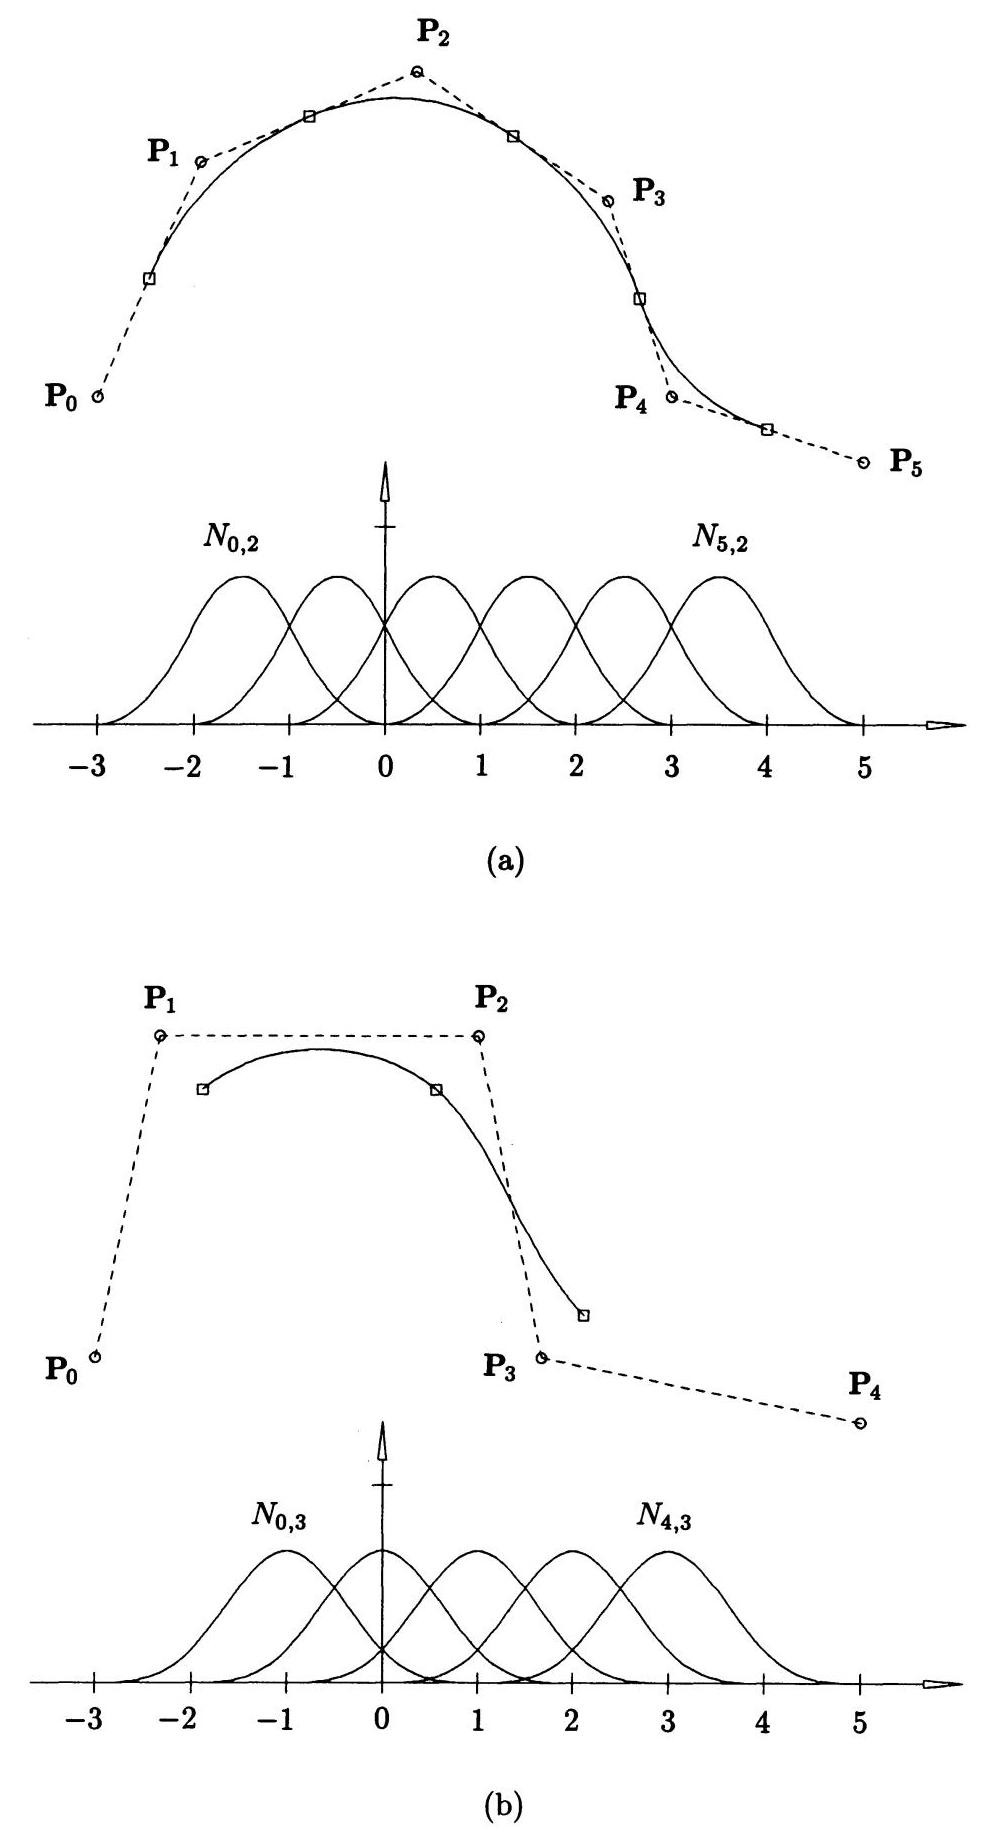
\includegraphics[max width=0.9\textwidth]{images/0193ba0d-ab19-7138-9798-cb281ce60de0_577_269_245_995_1837_0.jpg}
\end{center}
\hspace*{3em} 

图 12.1. 未夹紧的 NURBS 曲线。 (a) 二次曲线；(b) 三次曲线。

\begin{center}
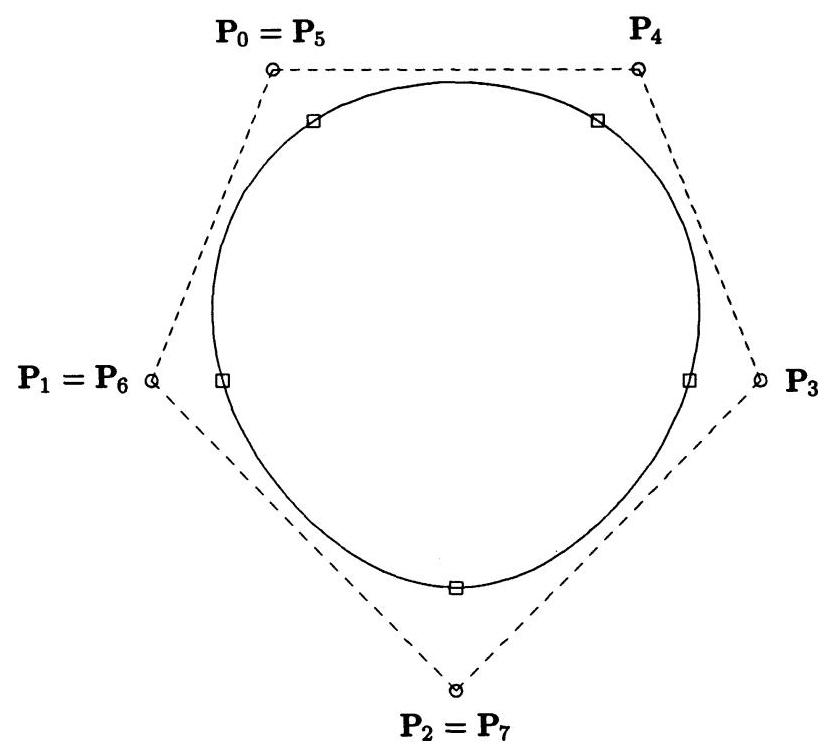
\includegraphics[max width=0.7\textwidth]{images/0193ba0d-ab19-7138-9798-cb281ce60de0_578_350_250_830_752_0.jpg}
\end{center}
\hspace*{3em} 

图 12.2. 闭合的 \({C}^{2}\) 连续未夹紧三次曲线。

之前所述的关于未固定的均匀曲线的所有内容同样适用于未固定的非均匀曲线，唯一的例外是闭合曲线的起始/结束处的 \({C}^{p - 1}\) 连续性。由于连续性依赖于节点值以及控制点位置，闭合的非均匀曲线的 \({C}^{p - 1}\) 连续性并不一定意味着控制点的精确包裹。图12.3a展示了在固定的均匀节点向量上定义的闭合立方曲线。

\[
U = \{ 3,3,3,3,4,5,6,7,8,8,8,8\}
\]

该曲线在起始/结束点处是 \({C}^{2}\) 连续的。图12.3b和 \({12.3}\mathrm{c}\) 显示了(精确地)相同曲线的未固定版本；图12.3b中的曲线使用了节点。

\[
U = \{ 0,{0.5},{2.3},3,4,5,6,7,8,{8.7},{10.5},{11}\}
\]

图12.3c中的曲线使用了节点。

\[
U = \{ 0,1,2,3,4,5,6,7,8,9,{10},{11}\}
\]

在这里重要的是指出，从算法的角度来看，固定曲线和未固定曲线之间几乎没有区别。只需稍作修改，本书前五章中给出的所有基本算法也可以用于未固定曲线。

在 CAD/CAM 的早期阶段(1980 年代初之前)，使用非均匀节点向量、夹紧或不夹紧的工作非常少。尽管在这个领域的术语一直令人困惑，早期的 CAD/CAM 工作者通常将 B 样条称为非周期性或周期性；非周期性与夹紧同义(如本书所述)，这些用于定义开放曲线和曲面(最初是均匀的，后来是非均匀的)。周期性在数学上等同于不夹紧、均匀，这些用于构造 \({C}^{p - 1}\) 连续封闭曲线和曲面。参考图 12.1a 和 12.1b，可以看到不夹紧、均匀的基函数都是彼此的平移，因此它们常被称为周期性。对于周期性 B 样条，不需要存储节点向量，不需要 Cox-deBoor 算法，也不需要控制点的环绕来获得 \({C}^{p - 1}\) 连续封闭曲线。一个简单的矩阵形式的(单个)基函数，加上一个特殊的控制点索引方案，就足以评估周期性 B 样条曲线(详见 [Mort85] 的讨论)。尽管更高效，这种对周期性 B 样条的特殊处理几乎在实践中消失，可能是因为软件开发和维护所需的时间已经变得比 CPU 时间昂贵得多。夹紧和不夹紧是较新的术语，可能会逐渐增多使用，仅仅因为它们更直观和准确。尽管在文献中这些术语出现得相对不频繁，但它们在 CAD/CAM 社区似乎相当普遍。我们在本书中使用非周期性这个术语，仅仅是因为我们尚未打破这个习惯。

\begin{center}
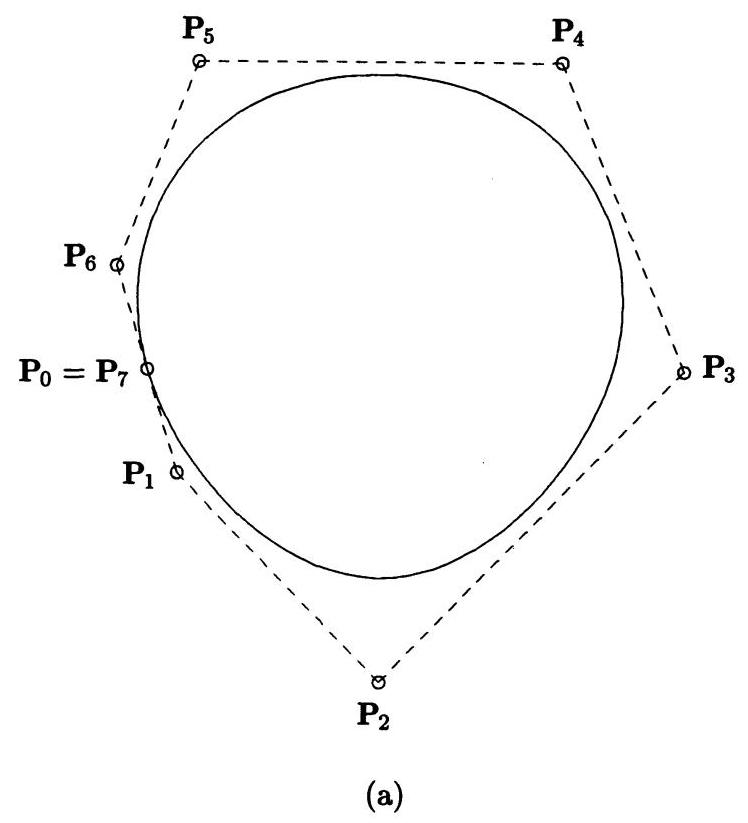
\includegraphics[max width=0.6\textwidth]{images/0193ba0d-ab19-7138-9798-cb281ce60de0_579_398_254_748_823_0.jpg}
\end{center}
\hspace*{3em} 

图 12.3. 使用不同节点向量解锁闭合曲线的示例。(a) 闭合夹紧曲线；(b) 无环绕解锁；(c) 带环绕解锁。

目前许多系统仅使用夹紧 B 样条。然而，IGES 和 STEP 都支持无夹紧 B 样条的交换。双向的精确转换都是可能的。夹紧曲线无非是将节点 \({u}_{p}\) 和 \({u}_{m - p}\) 插入，直到它们的重数达到 \(p\) ，然后丢弃位于夹紧区域之外的节点和控制点。节点插入公式(公式 (5.15))同样适用于无夹紧曲线，只要不对范围在 0 到 \(m\) 之外的节点进行索引(在 \({u}_{p}\) 和 \({u}_{m - p}\) 夹紧时不会发生这种情况)。我们建议(但留作练习)读者编写一个例程，以提取任意参数 \({u}_{1}\) 和 \({u}_{2}\) 之间的子曲线，其中 \({u}_{1} < {u}_{2}\) 。这样的例程不仅处理夹紧，还有许多其他用途，包括我们在下一节中提到的一个用途。

\begin{center}
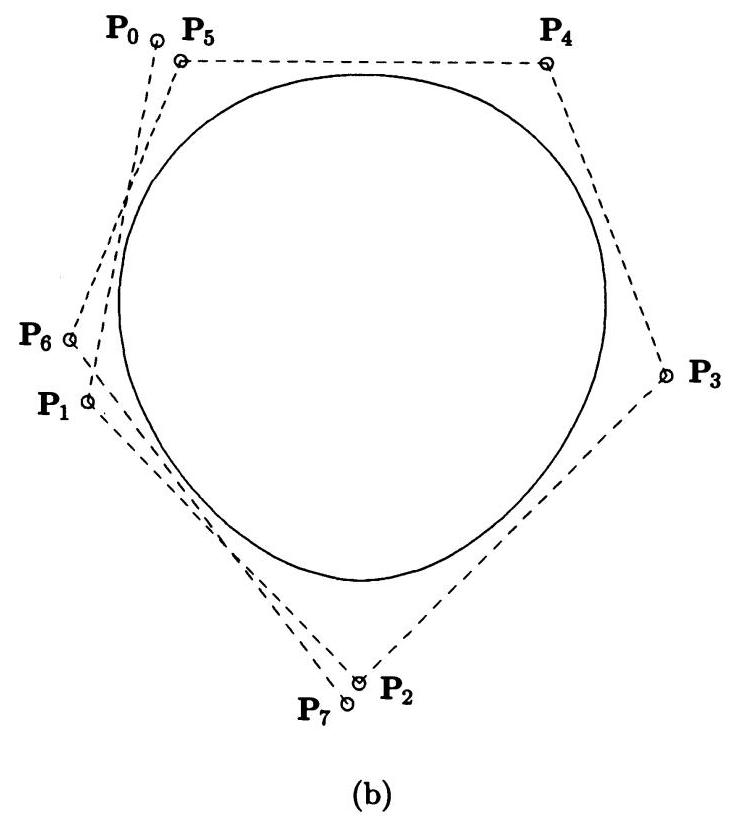
\includegraphics[max width=0.6\textwidth]{images/0193ba0d-ab19-7138-9798-cb281ce60de0_580_405_255_732_822_0.jpg}
\end{center}
\hspace*{3em} 

图 12.3.(续)

解锁本质上是节点移除。尽管解锁很少被要求(是的，确实有仅处理无夹紧 B 样条的系统)，我们在此呈现算法 A12.1，该算法计算每端的 \(p - 1\) 新控制点和每端的 \(p\) 新节点，所有操作均在原地进行。我们提醒读者，结果并不是唯一的(见图 12.3b 和 12.3c)。选择 \({2p}\) 新端节点是相对自由的，而新控制点的位置依赖于节点。我们选择新节点如下:

\[
{u}_{p - i - 1} = {u}_{p - i} - \left( {{u}_{n - i + 1} - {u}_{n - i}}\right) \;i = 0,\ldots ,p - 1 \tag{12.1}
\]

和

\[
{u}_{n + i + 2} = {u}_{n + i + 1} + \left( {{u}_{p + i + 1} - {u}_{p + i}}\right) \;i = 0,\ldots ,p - 1 \tag{12.2}
\]

这种节点选择会导致控制点的环绕，如图 12.2 和 \({12.3}\mathrm{c}\) 所示，前提是夹紧曲线以 \({C}^{p - 1}\) 连续性闭合。算法为:

\HRule

\hspace*{21em} <img src="https://cdn.noedgeai.com/0193ba0d-ab19-7138-9798-cb281ce60de0\_581.jpg?x=354\&y=248\&w=827\&h=744"/>

\hspace*{44em} (c)

\hspace*{10em} Figure 12.3. (Continued.)

\hspace*{13em} \#\# ALGORITHM A12.1

\hspace*{15em} UnclampCurve(n, p, U, Pw)

\hspace*{17em} \{ /* Unclamp a clamped curve */

\hspace*{20em} /* Input: n, p, U, Pw */

\hspace*{20em} /* Output: U, Pw */

\hspace*{17em} for (i=0; i<=p-2; i++) /* Unclamp at left end */

\hspace*{19em} \{

\hspace*{19em} \(U\left\lbrack  {p - i - 1}\right\rbrack   = U\left\lbrack  {p - i}\right\rbrack   - \left( {U\left\lbrack  {n - i + 1}\right\rbrack   - U\left\lbrack  {n - i}\right\rbrack  }\right) ;\)

\hspace*{19em} \(\mathrm{k} = \mathrm{p} - 1\) ;

\hspace*{19em} for (j=i; j>=0; j--)

\hspace*{21em} \{

\hspace*{21em} alfa = (U[p]-U[k])/(U[p+j+1]-U[k]);

\hspace*{21em} \(\operatorname{Pw}\left\lbrack  j\right\rbrack   = \left( {\operatorname{Pw}\left\lbrack  j\right\rbrack   - \operatorname{alfa} * \operatorname{Pw}\left\lbrack  {j + 1}\right\rbrack  }\right) /\left( {{1.0} - \operatorname{alfa}}\right) ;\)

\hspace*{21em} \(\mathrm{k} = \mathrm{k} - 1\) ;

\hspace*{21em} \}

\hspace*{19em} \}

\hspace*{17em} U[0] = U[1] - (U[n-p+2]-U[n-p+1]); /* Set first knot */

\hspace*{17em} for (i=0; i<=p-2; i++) /* Unclamp at right end */

\hspace*{19em} \{

\hspace*{19em} \(U\left\lbrack  {n + i + 2}\right\rbrack   = U\left\lbrack  {n + i + 1}\right\rbrack   + \left( {U\left\lbrack  {p + i + 1}\right\rbrack   - U\left\lbrack  {p + i}\right\rbrack  }\right) ;\)

\hspace*{19em} for (j=i; j>=0; j--)

\hspace*{21em} \{

\hspace*{3em} alfa = (U[n+1]-U[n-j])/(U[n-j+i+2]-U[n-j]);

\hspace*{3em} \(\mathrm{{Pw}}\left\lbrack  {\mathrm{n} - \mathrm{j}}\right\rbrack   = \left( {\mathrm{{Pw}}\left\lbrack  {\mathrm{n} - \mathrm{j}}\right\rbrack   - \left( {{1.0} - \mathrm{{alfa}}}\right)  * \mathrm{{Pw}}\left\lbrack  {\mathrm{n} - \mathrm{j} - 1}\right\rbrack  }\right) /\mathrm{{alfa}};\)

\hspace*{2em} \}

\hspace*{1em} \}

U[n+p+1] = U[n+p] + (U[2*p]-U[2*p-1]); /* Set last knot */

\}

\HRule

图 12.4a-12.4d 显示了对一个 4 次曲线的左端进行解夹的步骤。图 12.4b-12.4d 分别对应于 \(i\) 第 \(i = 0,1,2\) 步的完成。

\[
U = \left\{  {0,0,0,\frac{1}{4},\frac{1}{4},\frac{1}{2},\frac{1}{2},\frac{3}{4},\frac{3}{4},1,1,1}\right\}
\]

(见示例 Ex7.2)。九个控制点已被标记。图 12.5b 说明了通过算法 A12.1 解夹后的圆。注意，控制多边形并没有环绕，因为没有控制点重合。这是因为圆在齐次空间中仅是 \({C}^{0}\) 连续的。解夹后的节点向量为:

\[
U = \left\{  {-\frac{1}{4}, - \frac{1}{4},0,\frac{1}{4},\frac{1}{4},\frac{1}{2},\frac{1}{2},\frac{3}{4},\frac{3}{4},1,\frac{5}{4},\frac{5}{4}}\right\}
\]

\begin{center}
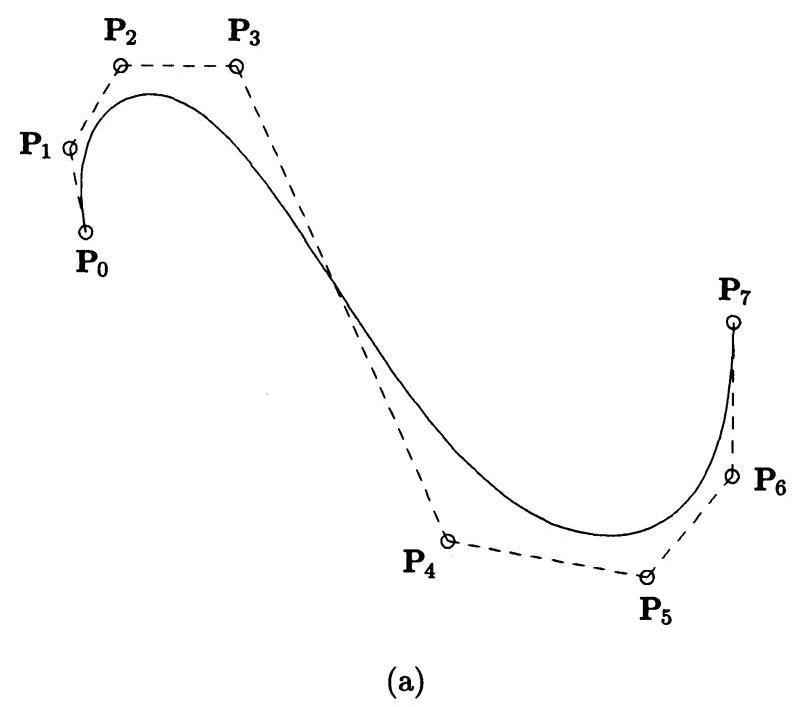
\includegraphics[max width=0.7\textwidth]{images/0193ba0d-ab19-7138-9798-cb281ce60de0_582_368_1311_796_707_0.jpg}
\end{center}
\hspace*{3em} 

图 12.4。对四次曲线左端进行解夹的过程。(a)原始夹紧曲线；(b)计算的 \(i = 0; \rightarrow  {\mathbf{P}}_{0}^{0}\) ；(c)计算的 \(i = 1; \rightarrow  {\mathbf{P}}_{0}^{1}\) 和 \({\mathbf{P}}_{1}^{1}\) ；(d)计算的 \(i = 2; \rightarrow  {\mathbf{P}}_{0}^{2},{\mathbf{P}}_{1}^{2}\) 和 \({\mathbf{P}}_{2}^{2}\) 。

显然，将这些结果扩展到曲面是直接的。通过将算法 A12.1 的计算应用于控制点的 \(m + 1\) 行 \(\left( {n + 1\text{ columns }}\right)\) ，可以在 \(u\left( v\right)\) 方向上对曲面进行解锁。图 12.6a-12.6d 显示了曲面解锁的示例。图 12.6a 显示了原始的度数为(3,2)的曲面。在图 12.6b 中展示了在 \(u\) 方向上的解锁，而在图 12.6c 中则展示了在 \(v\) 方向上的解锁。图 12.6d 显示了在两个方向上的解锁。

\begin{center}
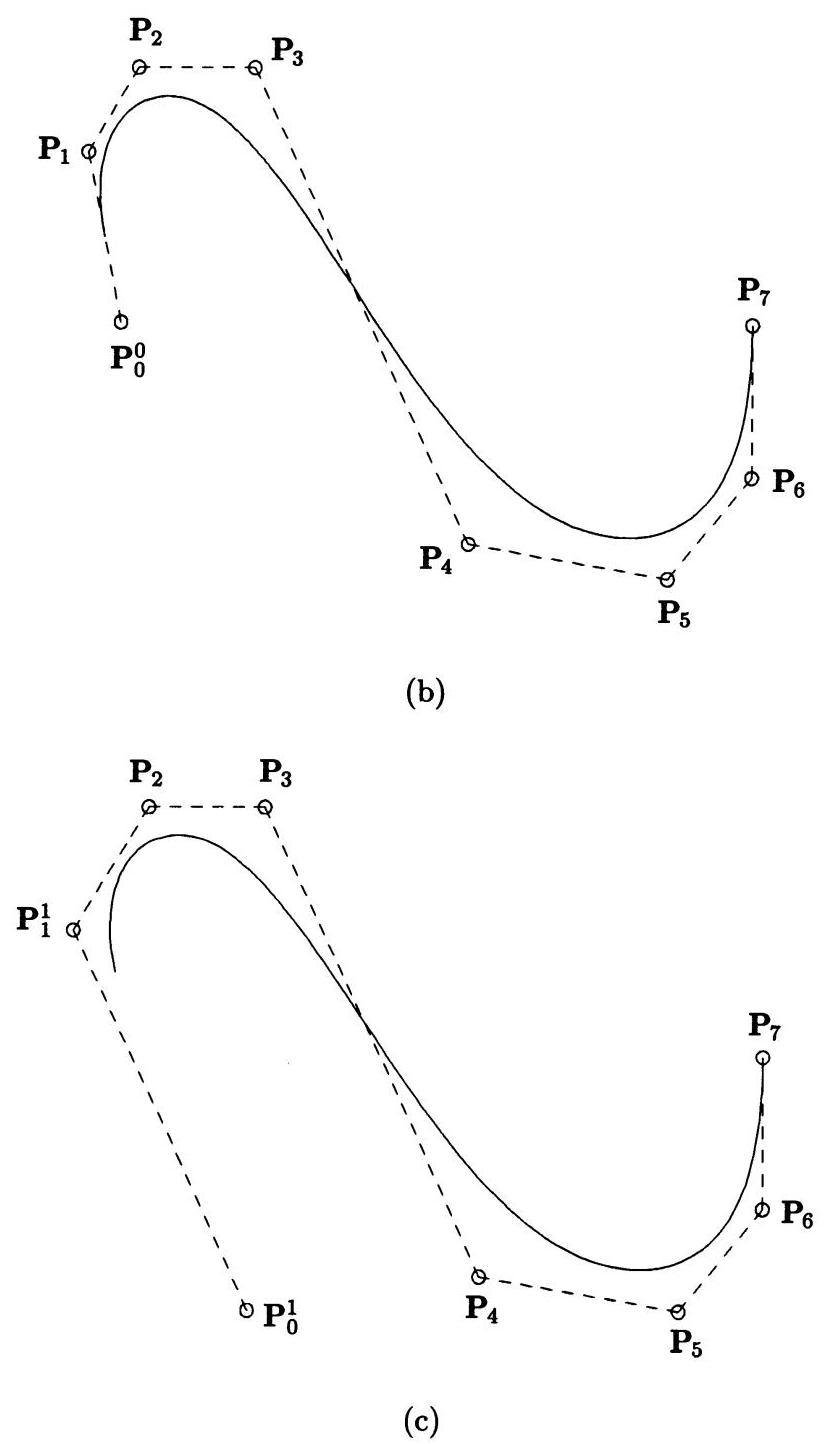
\includegraphics[max width=0.7\textwidth]{images/0193ba0d-ab19-7138-9798-cb281ce60de0_583_348_638_827_1444_0.jpg}
\end{center}
\hspace*{3em} 

图 12.4.(续)

\begin{center}
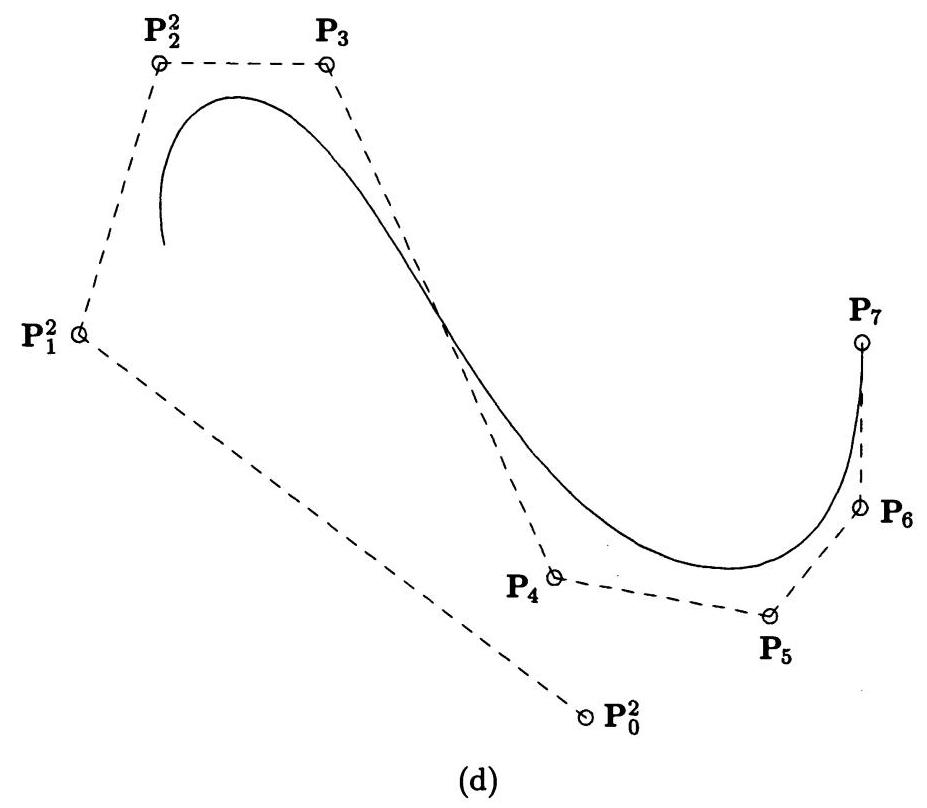
\includegraphics[max width=0.8\textwidth]{images/0193ba0d-ab19-7138-9798-cb281ce60de0_584_299_254_927_808_0.jpg}
\end{center}
\hspace*{3em} 

图 12.4.(续)



\section{标准中的 NURBS }

NURBS 不仅是 CAD/CAM/CAE 行业的事实标准，而且还被纳入了多个国际和美国国家标准:

\begin{itemize}
\item IGES:初始图形交换规范；
\end{itemize}

\begin{itemize}
\item STEP:产品模型数据交换标准；
\end{itemize}

\begin{itemize}
\item PHIGS:程序员的层次交互图形系统。
\end{itemize}

本节的主题是这些标准中 NURBS 的定义。目的是概念上传达每个标准中 NURBS 的定义。为此，我们采用非正式的风格，避免使用每个标准的具体术语。读者应查阅相关文件，以便对这些标准进行更严格的研究 [PHIG92; IGE93; STEP94]。有关进一步阅读，请参见 Bloor 和 Owen [Blor91] 以及 Vergeest [Verg91] 关于 STEP 的文献，以及 Howard [Howa91a] 和 Howard 等 [Howa91b] 关于 PHIGS 的文献。任何设计新 NURBS 系统的人都应确保其符合与 NURBS 相关的这些标准。


\subsection{IGES}

IGES(美国国家标准)是当今 CAD/CAM/CAE 系统中最广泛使用的产品数据交换格式。IGES 于 1980 年代初开发，规定了用于交换图形和几何数据的格式，支持各种应用，如制图、电路设计、有限元和管道设计。支持曲线、表面和三维固体。NURBS 曲线在 IGES 中的定义如下:

\begin{center}
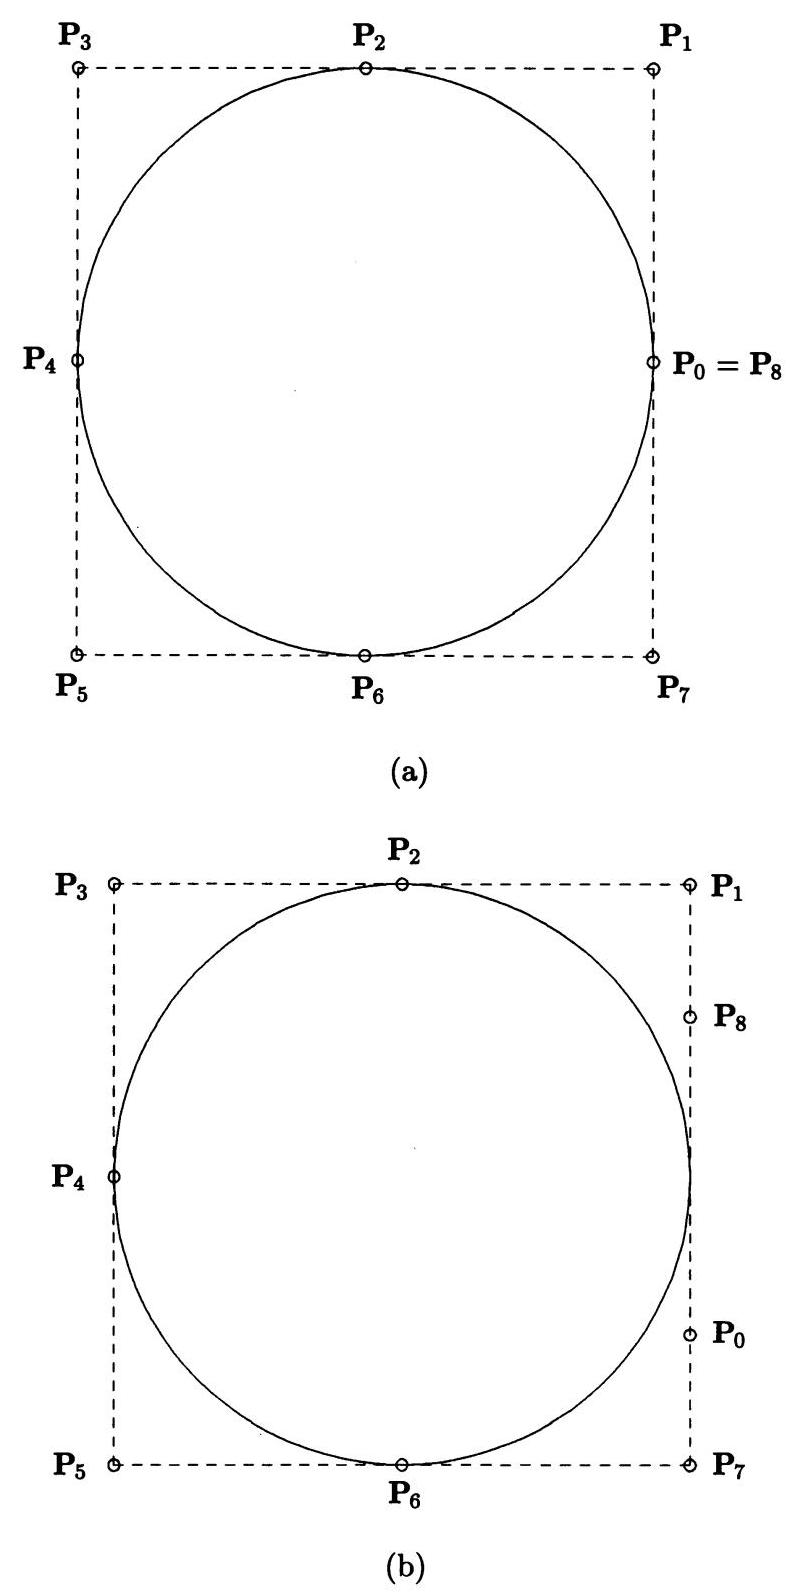
\includegraphics[max width=0.7\textwidth]{images/0193ba0d-ab19-7138-9798-cb281ce60de0_585_367_242_801_1592_0.jpg}
\end{center}
\hspace*{3em} 

图 12.5. 解锁九点 NURBS 圆。 (a) 原始曲线；(b) 解锁曲线。

\begin{center}
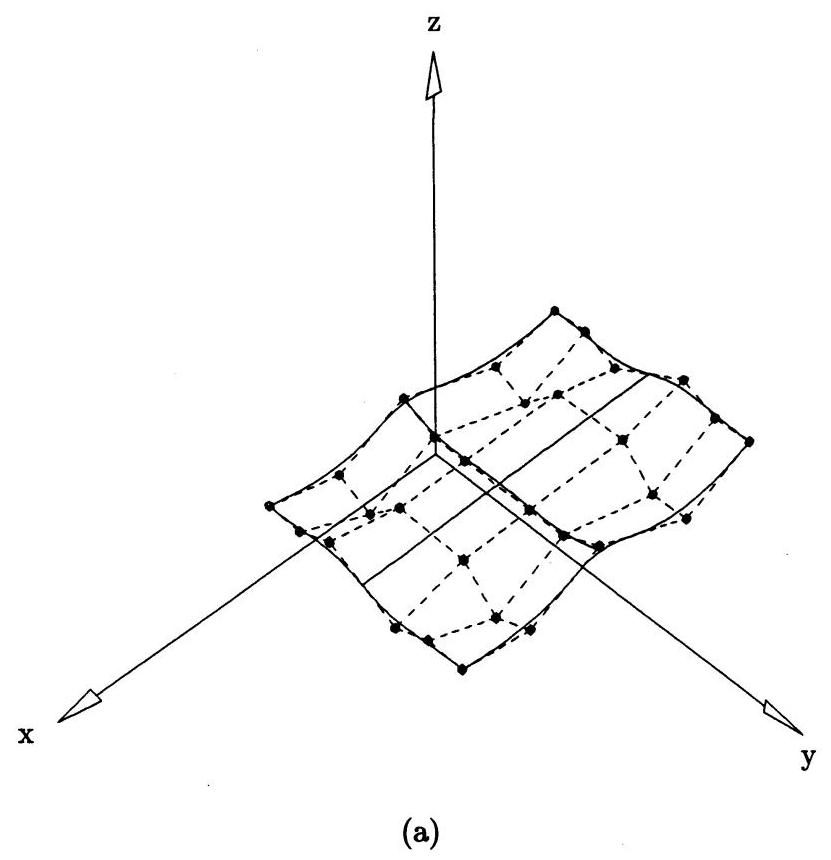
\includegraphics[max width=0.7\textwidth]{images/0193ba0d-ab19-7138-9798-cb281ce60de0_586_354_237_831_860_0.jpg}
\end{center}
\hspace*{3em} 

图 12.6. 解锁一个度数为 (3,2) 的表面。 (a) 原始表面；(b) 在 \(u\) 方向解锁；(c) 在 \(v\) 方向解锁；(d) 在两个方向解锁。

\begin{itemize}
\item 度数， \(p\) ，和控制点数量， \(n + 1\) ；
\end{itemize}

\begin{itemize}
\item 欧几里得控制点， \({\mathbf{P}}_{i}\) ，和权重， \({w}_{i}\) ；
\end{itemize}

\begin{itemize}
\item 一个包含 \(m + 1 = n + p + 2\) 个节点的节点向量， \(U\) ；
\end{itemize}

\begin{itemize}
\item 起始和结束参数值， \({s}_{0}\) 和 \({s}_{1}\) ；
\end{itemize}

\begin{itemize}
\item 其他非必要但有用的信息:曲线是平面还是非平面、开放还是封闭、真正有理( \({w}_{i}\) 不全相等)还是非有理、周期性还是非周期性；此外，曲线可以标记为特殊类型，例如直线、圆弧或圆锥弧。
\end{itemize}

注意，控制点和权重在 IGES 中是分开的项目；没有均匀控制点的概念， \({\mathbf{P}}_{i}^{w}\) 。仅允许正权重。“周期性”和“非周期性”这两个术语在 IGES 手册中没有定义，因此它们是没有意义的。它们通常被解释为分别表示未夹紧和夹紧，如第 12.2 节所定义。对节点的唯一约束是 \(m = n + p + 1\) 和 \({u}_{i - 1} \leq  {u}_{i}\) 对于 \(i = 1,\ldots ,m\) 。因此，几乎任何情况都是允许的，包括重数大于 \(p\) 的内部节点。参数 \({s}_{0}\) 和 \({s}_{1}\) 是定义的一个重要部分，因为它们定义了曲线的起点和终点。唯一的限制是 \({u}_{0} \leq  {s}_{0} < {s}_{1} \leq  {u}_{m}\) 。也就是说，预期的曲线可以是由节点 \({u}_{0},\ldots ,{u}_{m}\) 定义的较大曲线的一个适当子曲线。一个仅允许夹紧曲线且没有 \({s}_{0}\) 和 \({s}_{1}\) 值的系统可以通过应用子曲线提取来适应 IGES NURBS 曲线(包括未夹紧曲线)，这只是通过在 \({s}_{0}\) 和 \({s}_{1}\) 处插入节点来实现，使用算法 A5.1。

\begin{center}
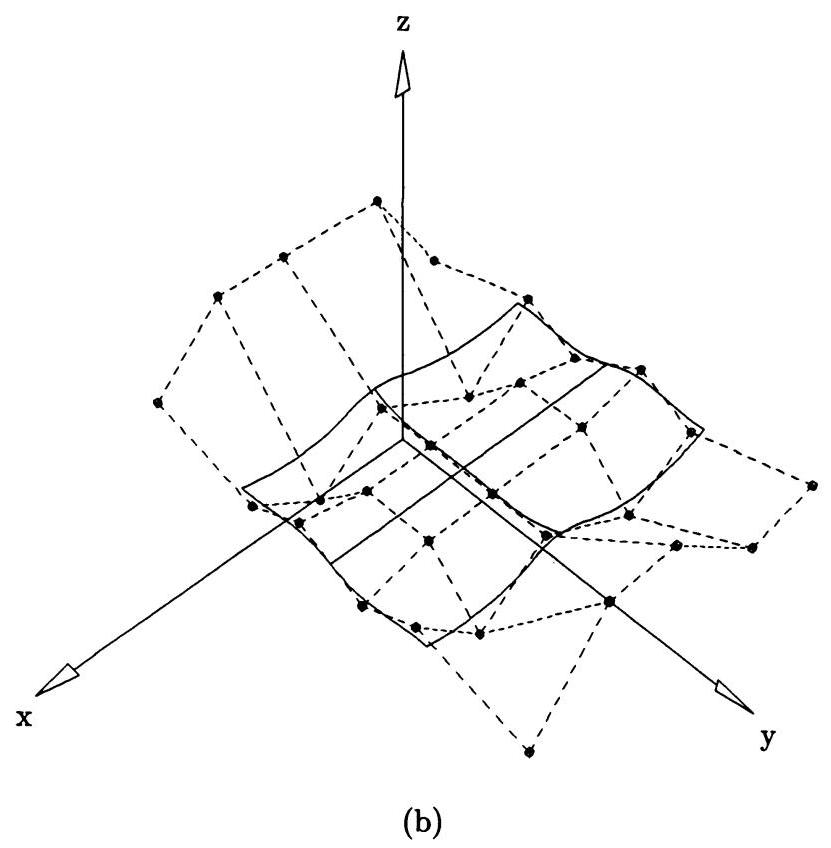
\includegraphics[max width=0.7\textwidth]{images/0193ba0d-ab19-7138-9798-cb281ce60de0_587_353_240_831_848_0.jpg}
\end{center}
\hspace*{3em} 

图 12.6.(续)

IGES NURBS 曲面是类比定义的。控制点和权重是分开的；权重必须为正。对 \(u\) 和 \(v\) 节点的唯一限制是 \(r = n + p + 1,s = m + q + 1,{u}_{i - 1} \leq  {u}_{i}\) 对于 \(i = 1,\ldots ,r\) 和 \({v}_{j - 1} \leq  {v}_{j}\) 对于 \(j = 1,\ldots ,s\) ，其中 \(p\) 和 \(n + 1\) ，以及 \(q\) 和 \(m + 1\) 分别是 \(u\) 和 \(v\) 方向上的度数和控制点数量。参数 \({s}_{0},{s}_{1}\) 和 \({t}_{0},{t}_{1}\) 定义了预期的曲面，该曲面可以是由给定节点、权重和控制点定义的曲面的适当子曲面。如果需要，使用节点插入来提取和限制预期的曲面。有信息标志指示曲面在每个方向上是开放还是封闭，以及是周期性 (?) 还是非周期性 (?)，以及曲面是否真正是有理的(所有 \({w}_{i,j}\) 相等)或非有理的。IGES NURBS 曲面可以标记为九种特殊类型之一:平面、圆柱、锥体、球体、环面、旋转曲面、一般柱面、规则曲面或一般二次曲面。



\subsection{STEP}
STEP 是一种新兴的国际标准，用于产品模型数据的交换。它代表了一项重大的国际努力，其复杂性、广度和深度远超 IGES。NURBS 曲线和曲面在所谓的第 42 部分中定义，该部分涉及产品模型的基本几何标准和数据交换及拓扑。实际上，由于 NURBS 表示法的通用性、数值稳定性和广泛的工业接受度，它被选为通过 STEP 交换一般样条和单跨度多项式及有理曲线和曲面的唯一方法。第 42 部分包括曲线、曲面和三维实体。NURBS 曲线在 STEP 中的指定方式为:

\begin{center}
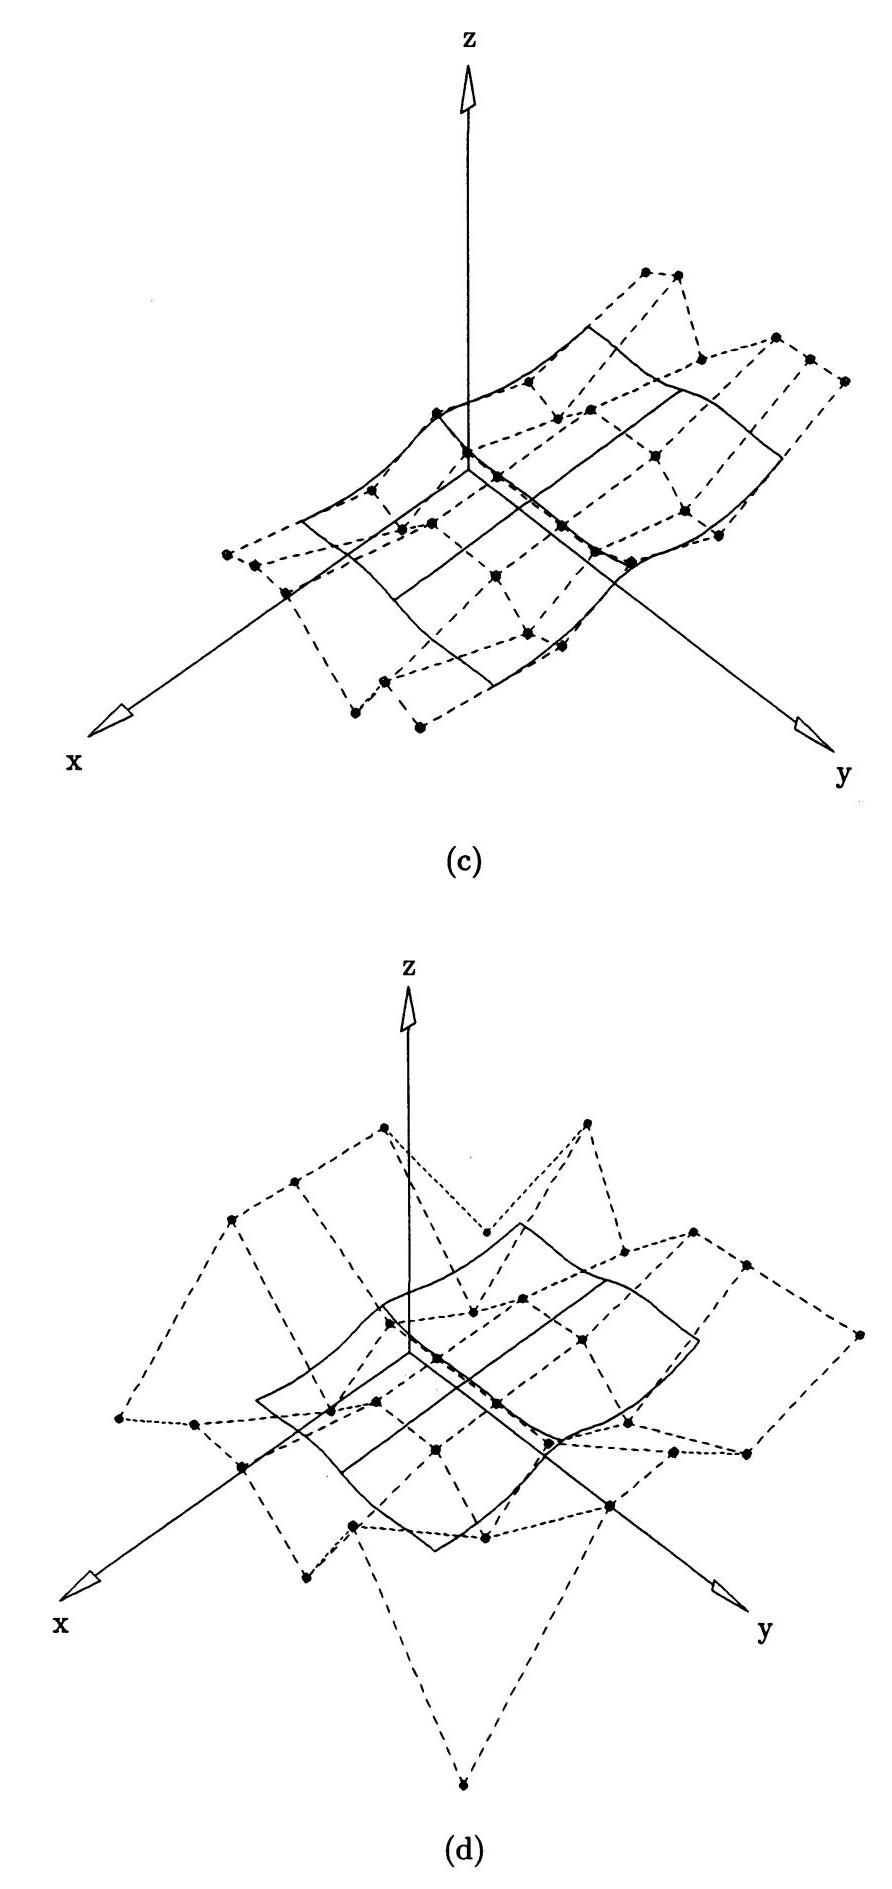
\includegraphics[max width=0.8\textwidth]{images/0193ba0d-ab19-7138-9798-cb281ce60de0_588_405_232_892_1889_0.jpg}
\end{center}
\hspace*{3em} 

图 12.6. (续)

\begin{itemize}
\item 度数， \(p\) 和控制点的数量， \(n + 1\) ；
\end{itemize}

\begin{itemize}
\item 欧几里得控制点， \({\mathbf{P}}_{i}\) 和权重， \({w}_{i}\) (没有 \({\mathbf{P}}_{i}^{w}\) 的概念)；仅允许正权重；
\end{itemize}

\begin{itemize}
\item 一个节点向量， \(U\) ，包含 \(m + 1 = n + p + 2\) 个节点，并满足 \({u}_{i - 1} \leq  {u}_{i}\) 对于 \(i = 1,\ldots ,m\) ；STEP 限制节点的重数 - 第一个和最后一个节点值的重数最多为 \(p + 1\) ，所有内部节点值的最大重数为 \(p\) ；
\end{itemize}

\begin{itemize}
\item 其他信息，例如节点向量的类型、曲线是开放的还是封闭的、是否自相交，以及如果适用的类型标签(折线、圆、圆锥)。
\end{itemize}

“修剪”曲线的概念通过参数 \({s}_{0}\) 和 \({s}_{1},{u}_{0} \leq  {s}_{0} < {s}_{1} \leq  {u}_{m}\) 存在于 STEP 中，但处于更高的层次；它并未嵌入曲线的定义中。STEP 根据节点向量的形式区分四种类型的 NURBS 曲线:均匀、准均匀、Bézier 和非均匀。如果 \({u}_{i} - {u}_{i - 1} = d\) 对于 \(i = 1,\ldots ,m\) 和某个正常数 \(d\) ，则节点向量是均匀的。这对应于第 12.2 节术语中的未夹紧和均匀。准均匀对应于夹紧和均匀，即 \({u}_{0} = \cdots  = {u}_{p},{u}_{m - p} =\)  \(\cdots  = {u}_{m}\) ，并且 \({u}_{i} - {u}_{i - 1} = d\) 对于 \(i = p + 1,\ldots ,m - p\) 和某个正常数 \(d\) 。Bézier 意味着不同的节点值均匀分布，并且第一个和最后一个具有重数 \(p + 1\) ，所有内部节点具有重数 \(p\) ，即曲线是分段 Bézier 的。任何不属于这三类的节点向量称为非均匀。

STEP NURBS 表面以类似方式定义。控制点和权重是分开的，权重必须为正。只有当其 \(u\) 和 \(v\) 节点均为各自类型时，表面才是均匀、准均匀或(分段)Bézier；否则它是非均匀的。存在自交标志，针对 \(u\) 和 \(v\) 方向的开放/封闭标志，以及(如适用)指示特殊类型的标签，如平面、圆柱、规则表面等。


\subsection{PHIGS}

尽管 IGES 和 STEP 是数据交换标准，但 PHIGS 是一个国际标准，指定了一个与设备无关的交互式图形编程接口。PHIGS 于1980年代中期出现，NURBS 于1992年作为 PHIGS PLUS 扩展的一部分被纳入该标准 [Howa91b]。支持 NURBS 的 PHIGS 实现允许应用程序员直接传递 NURBS 曲线和曲面以进行显示。NURBS 曲线在 PHIGS 中的定义如下:

\begin{itemize}
\item 阶数(= 度 + 1)、控制点数量和节点数量；
\end{itemize}

\begin{itemize}
\item 欧几里得控制点 \({\mathbf{P}}_{i}\) ，如果曲线是非有理的，则使用四维齐次控制点 \({\mathbf{P}}_{i}^{w}\) ；一个标志指示有理性。权重必须为正；
\end{itemize}

\begin{itemize}
\item 节点；仅允许使用夹紧节点向量，可以是均匀或非均匀的。节点的重数没有限制；
\end{itemize}

\begin{itemize}
\item 修剪参数 \({s}_{0}\) 和 \({s}_{1}\) ，定义预期曲线的实际起始和结束。
\end{itemize}

NURBS 曲面的定义类似，只是没有修剪参数。允许更一般的修剪循环，由曲面参数域中的 NURBS 曲线组成。



\section{NURBS 系统的数据交换}

在本节中，我们假设两个曲线和曲面系统 A 和 B，并研究它们之间的数据交换。我们假设系统 A 是基于本书设计和实现的，即它使用任意阶数的夹紧 NURBS 曲线和曲面。为了实用性和与大多数现有系统的兼容性，我们还要求所有权重为正，并且内部节点的重数不超过阶数。目前，我们对系统 B 中几何体的表示方式没有任何假设。

在两个以不同方式表示几何的系统之间交换曲线或曲面时，有三种可能的情况:

\begin{itemize}
\item 可以进行数学上精确的转换，这意味着浮点数舍入是唯一的误差。两种系统中的几何在几何和参数上都是等价的；一个例子是第 6.6 节中给出的 B-spline 和分段幂基形式之间的转换；
\end{itemize}

\begin{itemize}
\item 转换在几何上是精确的，但参数化发生了变化；一个例子是圆，在系统 B 中通过三角函数进行参数化。注意，如果圆用于在系统 A 和 B 中形成某些类型的曲面(例如规则曲面、皮肤曲面、戈登曲面和库恩斯曲面)，则得到的曲面几何可能会不同；
\end{itemize}

\begin{itemize}
\item 在数学上，两种系统之间不存在精确的转换；在这种情况下，最佳的做法是对某个指定的容差进行近似。例如，如果系统 B 仅允许三次曲线，则必须对来自系统 A 的高阶曲线进行近似。
\end{itemize}

出于我们的目的，我们区分两种类型的几何:

\begin{itemize}
\item 解析几何的简单曲线和曲面，如直线、圆、圆锥曲线、平面、圆柱或圆锥、球体和环面； - 其他一切。假设系统 B 可以表示解析类型，则在系统 A 和 B 之间的这些交换在两个方向上都是几何精确的。考虑从 B 到 A 的方向。大多数系统以有理形式(例如，有理幂基或贝塞尔)表示解析类型，或以易于推导几何特征(如中心、轴、半径、顶点等)的形式表示。第 6.6 节展示了如何将分段有理幂基或贝塞尔形式转换为 NURBS；从其他有理形式转换为 NURBS 也是类似的。从几何特征构建解析类型的 NURBS 表示是第 7 章和第 8 章的主题。将解析类型从系统 A 传递到 B 更为困难。问题在于曲线或曲面的 NURBS 表示并不是唯一的。例如，有无限多种组合的度数、节点、控制点和权重可以生成以原点为中心的完整单位圆。因此，确定 NURBS 曲线是否为解析类型并计算其几何特征并不简单。第 7.6 节提出了一种方法来确定二次有理贝塞尔曲线的几何特征。然而，可能需要进行度数降低和节点插入，以将 NURBS 曲线转换为分段二次有理形式(如果可能的话)。此外，只有当 NURBS 曲线在每个贝塞尔段上产生相同的几何特征(在公差范围内)时，它才是圆锥曲线。我们强调，我们仅对系统 A 中构成 NURBS 曲线或曲面的内容做出假设；我们对特定解析类型如何构建为 NURBS 不做任何假设。实际上，这种几何形状可能在另一个系统中以 NURBS 形式创建，但使用与本书中所呈现的节点、权重和控制点的不同组合，然后传递到系统 A。为 NURBS 几何提供类型标签，如 IGES 和 STEP 中允许的(见第 12.3 节)，在这方面提供了一些帮助；但这并不能消除问题。
\end{itemize}

现在考虑更复杂的几何形状，从一般的规则和旋转表面到偏移、混合、倒角以及一般自由形状的曲线和表面。系统 B 可能使用三种方法来表示这样的几何形状:

\begin{itemize}
\item 形式为 \(f\left( {x,y}\right)  = 0\) 或 \(f\left( {x,y,z}\right)  = 0\) 的隐式方程；
\end{itemize}

\begin{itemize}
\item 程序定义；
\end{itemize}

\begin{itemize}
\item 多项式或有理样条的多种形式之一。
\end{itemize}

理论上，可以使用被称为隐式化的技术将 NURBS 精确转换为分段隐式形式(例如，参见 [deMo84; Sede84; Hoff89] 及其中的参考文献)。然而，这在计算上并不实用；从隐式形式精确转换为 NURBS 形式通常是不可能的，因此需要近似。在实践中，隐式方程很少用于表示复杂几何，因此我们不再深入探讨这一主题。

如果一条曲线或表面不是通过显式系数或函数直接定义，而是通过其他基曲线或表面间接定义，并结合一个程序或公式从基几何上的点计算出目标几何上的点，则我们称其为程序定义。

偏移曲线和表面是程序定义几何的例子。偏移表面 \(\mathbf{O}\left( {u,v}\right)\) 由以下方式指定:

\[
\mathbf{O}\left( {u,v}\right)  = \mathbf{S}\left( {u,v}\right)  + d\mathbf{N}\left( {u,v}\right)  \tag{12.3}
\]

其中 \(\mathbf{S}\left( {u,v}\right)\) 是基表面， \(d \neq  0\) 是一个常数标量，而 \(\mathbf{N}\left( {u,v}\right)\) 是 \(\mathbf{S}\left( {u,v}\right)\) 在 (u, v) 处的单位长度法向量。偏移曲线和表面在数学上是复杂的，通常很难精确表示为 NURBS 形式(参见 [Till84; Faro86; Coqu87b; Hosc88])。混合和倒角表面有时是通过程序定义的 [Choi91]，而 Filip 和 Ball [Fili89] 描述了一种皮肤化的程序方法。这些表面很少能够在没有近似的情况下传递到 NURBS(或任何其他)系统中。

大多数 CAD/CAM/CAE 系统使用分段多项式或有理曲线和曲面来表示复杂几何。我们统称这些为样条曲线。样条曲线有许多不同类型；但无论它有什么华丽的名称，样条曲线(曲面)仅由若干段(补丁)组成，这些段以某种形式的连续性拼接在一起。为了简洁起见，我们在本节的其余部分将讨论限制于曲线，但类似的陈述和算法也适用于曲面。为了确定特定类型的样条曲线是否具有等效的 NURBS 表示(反之亦然)，必须考虑三件事:

\begin{itemize}
\item 度数；
\end{itemize}

\begin{itemize}
\item 有理性；
\end{itemize}

\begin{itemize}
\item 连续性。
\end{itemize}

度数和有理性是简单的。度数可以精确提高，但不能降低；而多项式是有理函数，但反之则不成立。由于我们的系统 A 允许任意度数的有理曲线，因此在将几何从系统 B 引入系统 A 时在这方面没有问题。然而，如果系统 B 限制度数或仅允许非有理几何，那么在从系统 A 转到系统 B 时，必须对相应的曲线进行近似。

连续性更为复杂。设 \(\mathbf{C}\left( u\right)\) 为由区间 \(\left\lbrack  {{u}_{i - 1},{u}_{i}}\right\rbrack\) 上的线段 \({\mathbf{C}}_{i}\left( u\right) ,i = 1,\ldots ,m.{\mathbf{C}}_{i}\left( u\right)\) 组成的样条曲线，其中 \({u}_{0} < {u}_{1} < \cdots  < {u}_{m - 1} < {u}_{m}\) 。我们称 \(\left\{  {u}_{i}\right\}\) 为断点；如果 \(\mathbf{C}\left( u\right)\) 处于 B-spline 形式，则 \(\left\{  {u}_{i}\right\}\) 为不同的节点值。每对线段 \({\mathbf{C}}_{i}\left( u\right)\) 和 \({\mathbf{C}}_{i + 1}\left( u\right)\) 以某种类型和顺序的连续性连接，而数据交换中的基本问题始终归结为接收系统是否能够表示与适当连续性连接的线段。我们所说的连续性类型是指参数连续性 (C) 与几何连续性 (G)；有关几何连续性和各种构造以具有 \(G\) 连续性的样条的更多细节，请参见第 9.3.1 节以及 [Bars89, 90; Hosc93] 和其中的参考文献。我们提醒读者:

\begin{itemize}
\item \({G}^{1}\) 在 \({u}_{i}\) 处的连续性意味着一阶导数向量 \({\mathbf{C}}_{i}^{\prime }\left( {u}_{i}\right)\) 和 \({\mathbf{C}}_{i + 1}^{\prime }\left( {u}_{i}\right)\) 指向相同的方向，但可以具有不同的大小；
\end{itemize}

\begin{itemize}
\item 对于 B-spline，节点的重数表示基函数的连续性，这通常是曲线在均匀条件下的参数连续性；
\end{itemize}

\HRule

space;

\HRule

\begin{itemize}
\item 曲线段的重新参数化会改变其与邻近段的参数连续性，但不会改变其几何连续性。
\end{itemize}

由于系统 A 允许任意的节点间距和重数，它能够精确地、几何地和参数化地表示几乎所有至少是 \({C}^{0}\) 连续的多项式和有理样条曲线。然而，从 A 转到 B 可能需要对段进行近似或重新参数化(这不会改变整体曲线的几何形状)。例如，如果系统 B 使用有理 B 样条但不允许多个内部节点，则必须对具有双内部节点的 \({C}^{p - 2}\) 连续 B 样条曲线进行近似。如果系统 B 允许多个节点但要求不同的节点(断点)均匀分布，则系统 A 的所有曲线可以在几何上精确地传递到系统 B；然而，这需要重新参数化，并且在此过程中参数连续性会丧失。算法为:

1. 插入所有内部节点，直到它们的重数达到 \(p\) ，从而获得分段贝塞尔曲线；这将产生系统 B 中曲线的控制点；

2. 设

\[
d = \frac{{u}_{m} - {u}_{0}}{m}
\]

并定义系统 B 的节点向量为

\[
U = \{ \underset{p + 1}{\underbrace{{u}_{0},\ldots ,{u}_{0}}},\underset{p}{\underbrace{{u}_{1},\ldots ,{u}_{1}}},\ldots ,\underset{p}{\underbrace{{u}_{m - 1},\ldots ,{u}_{m - 1}}},\underset{p + 1}{\underbrace{{u}_{m},\ldots ,{u}_{m}}}\}
\]

其中

\[
{u}_{i} = {u}_{0} + i \cdot  d\;i = 1,\ldots ,m - 1
\]

3. 应用节点移除(至零容忍)，但所有断点的重数必须至少为一，以确保它们均匀分布。

注意，如果使用此算法将曲线从 A 传递到 B 然后再返回到 \(A\) ，则原始曲线和返回的曲线在 \(A\) 中在参数上和节点数量上是不同的。还要注意，尽管曲线在几何上是等价的，但如果它们在系统 A 中用于构造规则曲面(例如)，则生成的曲面可能在几何上并不等价。

无论系统 B 中使用何种类型的样条，连续性问题由两个部分组成:

\begin{itemize}
\item 表示是否允许不均匀间隔的断点；
\end{itemize}

\begin{itemize}
\item 可能的连续性类型和阶数是什么？
\end{itemize}

我们指出，即使在没有全局断点概念的系统中，第一部分的问题也可以得到回答。例如，许多几何连续样条是通过局部方法构造的，使用每个段的局部参数 \(t,t \in  \left\lbrack  {0,1}\right\rbrack\) 。这样的系统可能允许全局参数化，在这种情况下，全局断点 \({u}_{i}\) 是可用的，并且很可能允许非均匀间距。在没有全局参数化概念的系统中，隐含了均匀间隔的全局断点。如前所述，重新参数化可以用于将非均匀间隔的断点转换为均匀间隔的断点；然而，在此过程中，参数连续性会发生变化。相反，重新参数化将均匀间隔的断点转换为非均匀间隔的断点在将(几何上精确地)连续样条转换为连续 B 样条 \({G}^{k}\) 时是有用的(例如，这在第 9.3.2 节，方程 [9.37]-[9.39] 中进行了)。关于第二部分，必须确定允许的最小连续性阶数。例如，基于五次 \({G}^{2}\) 连续样条的系统可以表示所有五次 \({G}^{k}\) 连续样条，对于 \(k \geq  2\) ；然而，具有 \(k < 2\) 的五次 \({G}^{k}\) 连续样条必须被近似。作为另一个例子，仅允许单个内部节点的 B 样条系统的曲线是 \({C}^{p - 1}\) 连续的。因此，所有连续性阶数都是可能的，但其度数必须至少比所需的最小连续性高一个(即，最小连续性阶数可能取决于度数)。

我们现在总结系统 A 和 B 之间样条曲线的交换。所有至少是 \({C}^{0}\) 连续的样条曲线都可以精确(几何和参数上)地从系统 B 传递到 A。对于 \(G\) 连续曲线，多个节点是必要的，但如果需要，可以使用重新参数化来实现 \(C\) 连续性并降低内部节点的重数。在某些类型的表面构造(例如，规则表面)中使用重新参数化曲线可以改变表面几何。一个典型的转换算法首先计算每个段的幂基或贝塞尔系数，然后应用第 6.6 节的技术来构建 NURBS 表示。

从系统 A 到系统 B 的转换可能更为复杂。算法 A12.2 给出了确定这种转换应如何进行的逻辑思维过程。将 \(p\) 次 NURBS 曲线表示为 \(\mathbf{C}\) ，并假设系统 B 可以表示 \(k\) 次的样条，其中 \({p}_{\min } \leq  k \leq  {p}_{\max }\) 。

\HRule

ALGORITHM A12.2

\hspace*{1em} if (C is rational and System B only represents polynomials)

\hspace*{2em} \{

\hspace*{2em} Approximate \(\mathrm{C}\) ;

\hspace*{2em} return;

\hspace*{2em} \}

\hspace*{1em} if \(\left( {p > {p}_{\max }}\right)\)

\hspace*{2em} \{

\hspace*{2em} Approximate \(\mathbf{C}\) ;

\hspace*{2em} return;

\hspace*{2em} \}

\hspace*{1em} if \(\left( {p < {p}_{\min }}\right)\)

\hspace*{2em} \{

\hspace*{2em} DegreeElevateCurve \(\left( \mathbf{C}\right) ;\;\) /* to degree \({p}_{\min } *\) /

\hspace*{2em} return;

\hspace*{1em} \}

Let \(m\) be the minimum order continuity allowed in System B

\hspace*{1em} for a degree \(p\) curve.

Determine the minimum order, \(k\) , of continuity at any

\hspace*{1em} breakpoint of \(\mathbf{C}\) .

if \(\left( {k < m}\right)\)

\hspace*{1em} \{

\hspace*{1em} Approximate \(\mathrm{C}\) ;

\hspace*{1em} return;

\hspace*{1em} \}

Extract the segments of \(\mathbf{C}\) (knot insertion), and convert them

\hspace*{1em} to the segment coefficients required by System B

\hspace*{1em} (reparameterization may be necessary).

If applicable, load the global breakpoints into System B.

\HRule

确定最小连续性值 \(m\) 和 \(k\) 需要详细说明。存在 \(C\) 连续性和 \(G\) 连续性，对于有理曲线，均匀空间中的连续性与欧几里得空间中的连续性是不同的。值 \(m\) 和 \(k\) 必须指代系统 B 的样条所基于的连续性类型。例如，假设系统 B 使用有理 \({G}^{2}\) 连续样条。该样条基于欧几里得空间中的切线和曲率连续性，因此值 \(k\) 必须基于系统 A 的 NURBS 曲线在欧几里得空间中的 \(G\) 连续性。注意，示例 Ex7.2 中的二次完整圆在系统 B 中可以精确表示为 \({G}^{2}\) 样条，尽管作为 NURBS 曲线，它在欧几里得空间中仅是 \({C}^{1}\) 连续的，并且在均匀空间中甚至存在尖点。

我们以这样的观察结束本章:NURBS 形式不仅是一种强大而灵活的曲线和曲面设计方法，而且显然是今天最适合用于复杂曲线和曲面数据交换的表示方式。



\clearpage
    


\end{document}


